%%% Local Variables:
%%% mode: latex
%%% TeX-master: "../../report"
%%% End:

Tha main difference of NGCF \cite{wang2019neural} and NCF is the ""embedding propagation layers"" which are 
designed to incorporate collaborative signals.
This is achieved by including the information about high-order connectivities 
in users-items connections graph into embeddings of users and items \ref{fig:ngcf}.
This information isn't used explicitly in other methods, therefore this type 
of architectue is supposed to improve the quality of recommendations.
Specifically, each layer of embbedding propagation layers corresponds 
to the distance between user and item interaction. It produces messages which 
are passed between these graph nodes, are summed and then transformed to the 
embedding at this level.
\begin{figure}[h]
    \centering
    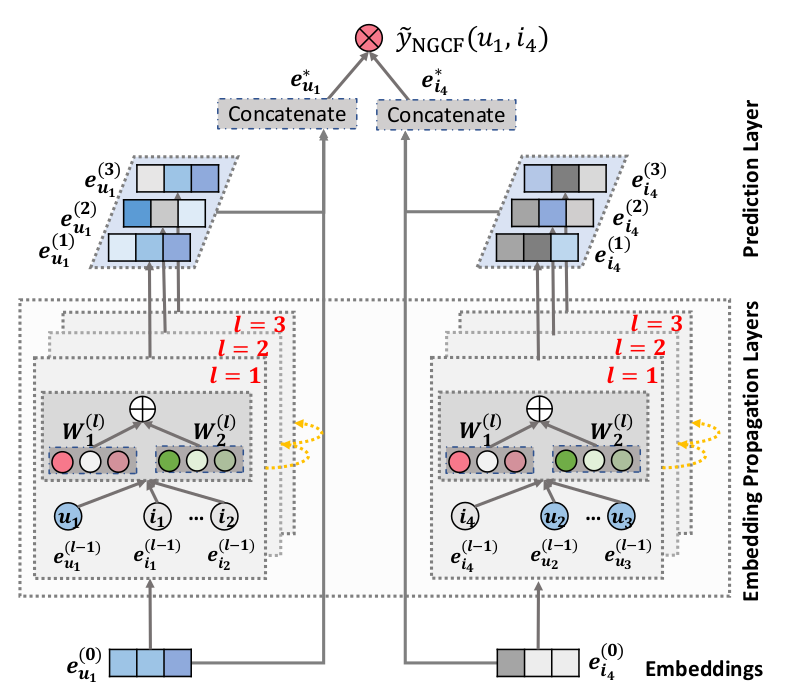
\includegraphics[width=0.8\linewidth]{images/ngcf.png}
    \caption{NGCF architecture taken from \cite{wang2019neural}}
    \label{fig:ngcf}
\end{figure}
In the end all the embeddings for each level are concatenated in order to produce a final embedding.
This embedding plays the role of latent vectors which can simply be multiplied in order to obtain the rating.
The model is trained using pairwise BPR loss and optimized using Adam.